\section{Gameplay}\label{sec:gameplay}
After the game is started, the user can finally start playing.
At the start, the screen will look like in \autoref{fig:gameplay}.
The user can see their position in the top left corner, the current frames per second in the top right corner, and the inventory in the bottom of the screen.
In the middle of the screen, there is a crosshair that shows where the user is aiming.
The user can also see their character model.
By using the controls described in \autoref{sec:controls}, the user can start moving around and exploring the world.


\begin{figure}[!htb]
    \centering
    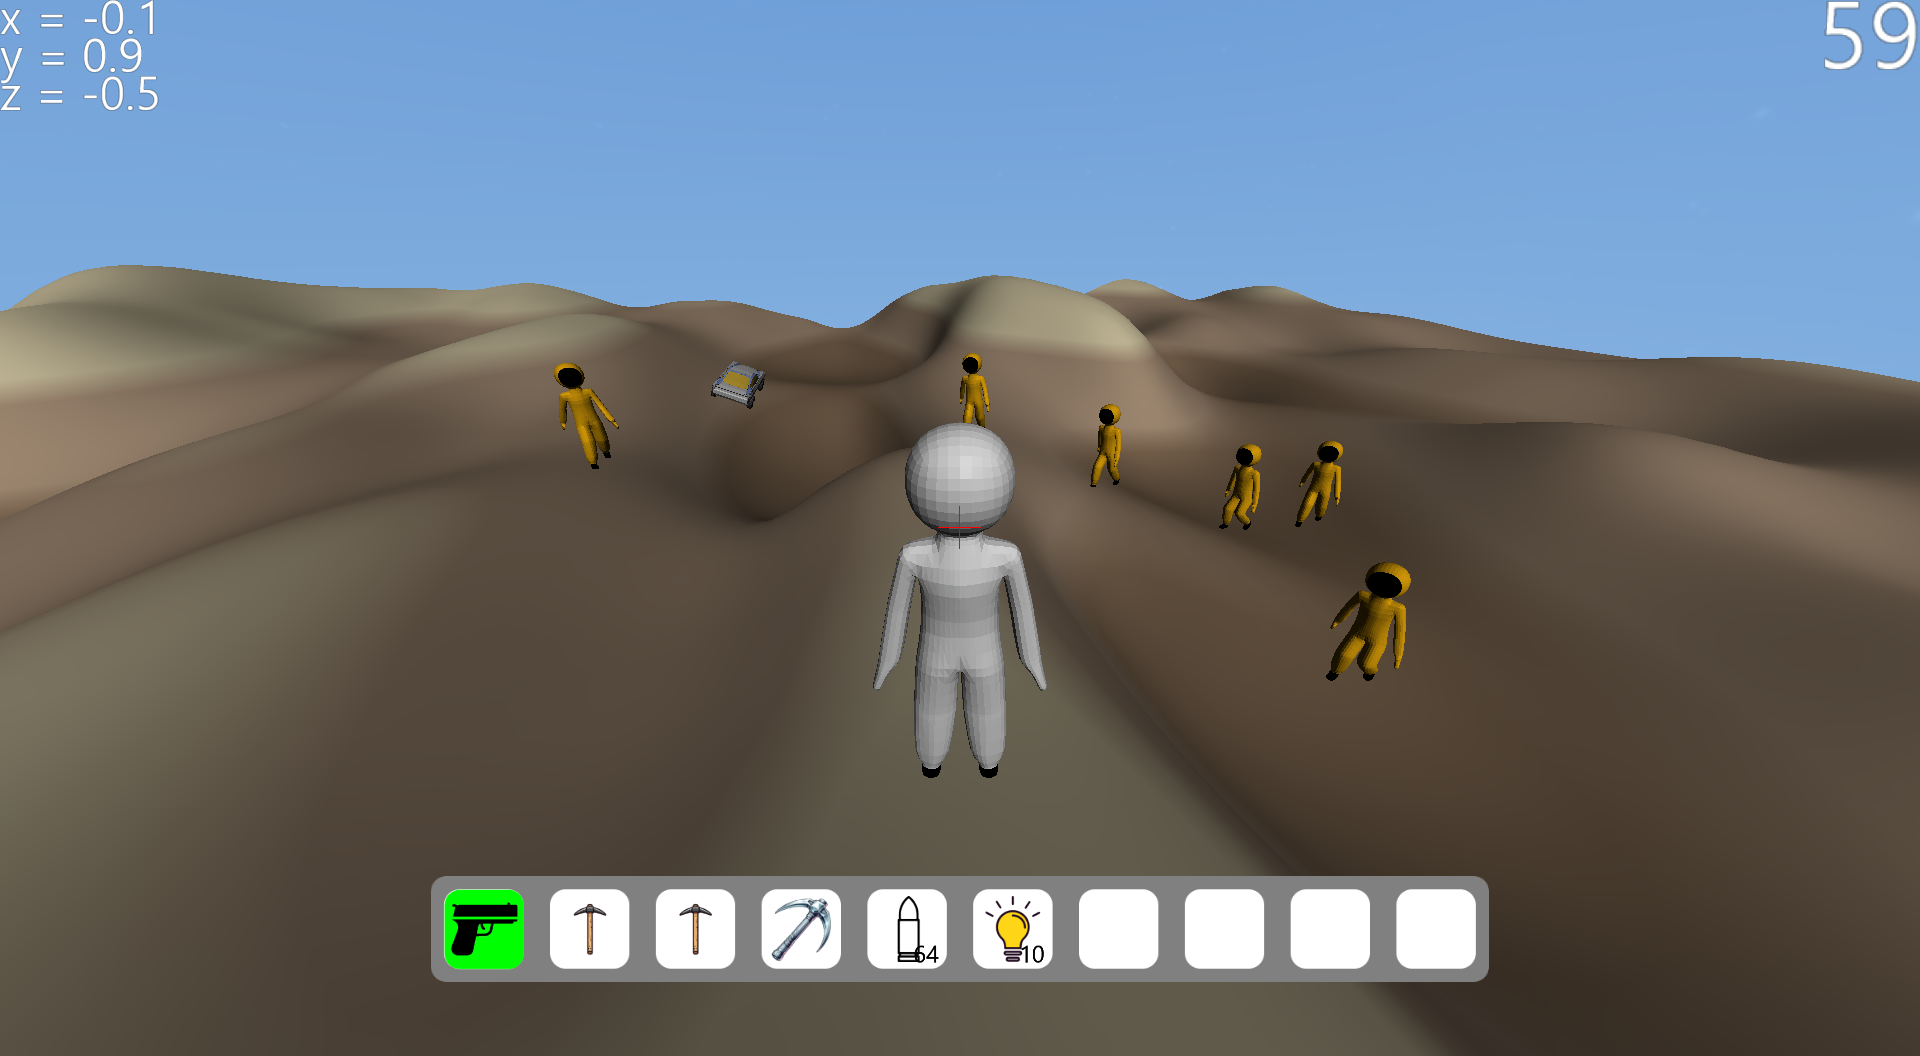
\includegraphics[width=0.8\textwidth]{chapters/user_manual/resources/gameplay.png}
    \caption{Controls screen}
    \label{fig:gameplay}
\end{figure}